\documentclass[11pt,a4paper]{article}

\usepackage[margin=1in]{geometry}
\usepackage{amsmath,amssymb,amsthm}
\usepackage{tikz}
\usetikzlibrary{calc,arrows.meta,decorations.markings}
\usepackage{pgfplots}
\pgfplotsset{compat=1.18}
\usepackage{enumitem}
\usepackage{booktabs}
\usepackage{hyperref}
\hypersetup{colorlinks=true,linkcolor=blue!60!black,citecolor=blue!60!black,urlcolor=blue!60!black}
\usepackage{xcolor}

\definecolor{pent1}{HTML}{7F77DD}
\definecolor{pent2}{HTML}{1D9E75}
\definecolor{pent3}{HTML}{D85A30}
\definecolor{vecred}{HTML}{E24B4B}

\newcommand{\vv}[1]{\mathbf{#1}}
\newcommand{\uv}[1]{\hat{\mathbf{#1}}}

\theoremstyle{definition}
\newtheorem{definition}{Definition}
\newtheorem{theorem}{Theorem}

\title{\bfseries Computing the Dihedral Angle\\of the Regular Dodecahedron}
\author{An Educational Derivation via Pentagon Folding}
\date{}

\begin{document}
\maketitle

\begin{abstract}
We compute the dihedral angle of the regular dodecahedron by studying how three
pentagonal faces meet at a common vertex. By folding two adjacent pentagons about
their shared edges with a central pentagon, we set up a system of equations using
Rodrigues' rotation formula and solve for the folding angle both numerically and
analytically. The result is the classical dihedral angle
$\pi - \arctan 2 \approx 116.57^\circ$, derived from the golden-ratio geometry of
the regular pentagon.
\end{abstract}

\tableofcontents
\vspace{1em}

%% ===================================================================
\section{Introduction}
%% ===================================================================

A \emph{regular dodecahedron} is one of the five Platonic solids, composed of twelve
congruent regular pentagonal faces, with three faces meeting at every vertex. A
fundamental geometric property of any polyhedron is its \emph{dihedral angle}---the
angle between two faces sharing an edge, measured in the plane perpendicular to that
edge.

For the regular dodecahedron, the dihedral angle is
\[
  \delta = \pi - \arctan 2 \approx 116.565^\circ.
\]
In this article, we derive this result from first principles by considering three
pentagonal faces that share a common vertex, then ``folding'' them out of their
initial plane until they close up into the configuration of a dodecahedron.

%% ===================================================================
\section{The Three-Pentagon Configuration}
%% ===================================================================

Consider three congruent regular pentagons lying flat in the $xy$-plane, all sharing
a common vertex at the origin, which we label $O$ (Figure~\ref{fig:pentagons}).

\begin{itemize}[nosep]
  \item \textbf{Pentagon~1} (central, purple) shares edge $OA$ with Pentagon~2 and
        edge $OB$ with Pentagon~3.
  \item \textbf{Pentagon~2} (teal) has edges $OA$ and $OC$ emanating from $O$.
  \item \textbf{Pentagon~3} (coral) has edges $OB$ and $OD$ emanating from $O$.
\end{itemize}

\begin{figure}[ht]
\centering
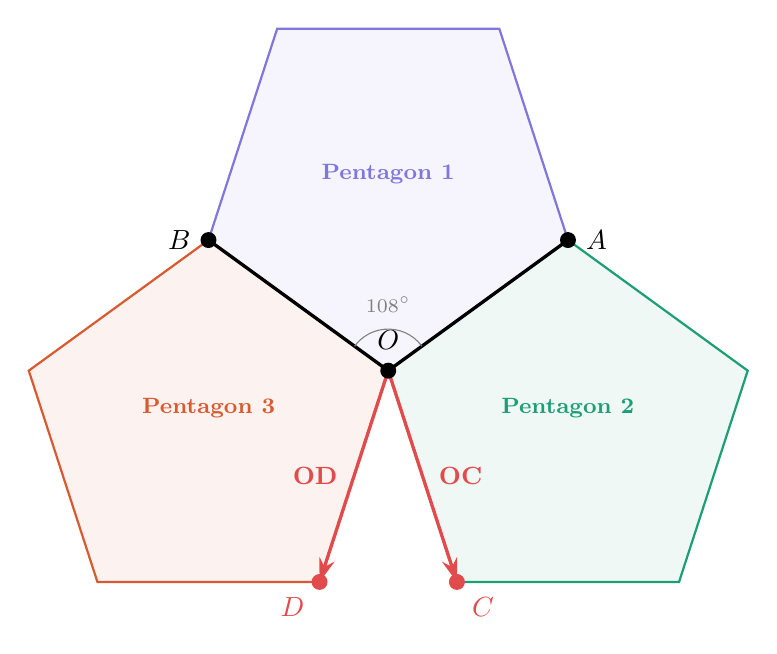
\begin{tikzpicture}[scale=2.4, >=Stealth,
  every node/.style={font=\small}]

% All coordinates precomputed from the exact pentagon geometry.
% O at origin; Pentagon 1 opens upward; Pentagons 2 and 3 fold downward.
\coordinate (O)   at ( 0.0000,  0.0000);
\coordinate (A)   at ( 0.9511,  0.6910);
\coordinate (B)   at (-0.9511,  0.6910);
\coordinate (C)   at ( 0.3633, -1.1180);
\coordinate (D)   at (-0.3633, -1.1180);

% Pentagon 1: O -- A -- P1b -- P1c -- B
\coordinate (P1b) at ( 0.5878,  1.8090);
\coordinate (P1c) at (-0.5878,  1.8090);

% Pentagon 2: A -- O -- C -- P2b -- P2c
\coordinate (P2b) at ( 1.5388, -1.1180);
\coordinate (P2c) at ( 1.9021,  0.0000);

% Pentagon 3: O -- B -- P3b -- P3c -- D
\coordinate (P3b) at (-1.9021,  0.0000);
\coordinate (P3c) at (-1.5388, -1.1180);

% --- Draw Pentagon 1 (purple) ---
\fill[pent1, opacity=0.07] (O) -- (A) -- (P1b) -- (P1c) -- (B) -- cycle;
\draw[pent1, thick]        (O) -- (A) -- (P1b) -- (P1c) -- (B) -- cycle;

% --- Draw Pentagon 2 (teal) ---
\fill[pent2, opacity=0.07] (A) -- (O) -- (C) -- (P2b) -- (P2c) -- cycle;
\draw[pent2, thick]        (A) -- (O) -- (C) -- (P2b) -- (P2c) -- cycle;

% --- Draw Pentagon 3 (coral) ---
\fill[pent3, opacity=0.07] (O) -- (B) -- (P3b) -- (P3c) -- (D) -- cycle;
\draw[pent3, thick]        (O) -- (B) -- (P3b) -- (P3c) -- (D) -- cycle;

% --- Shared edges (bold black) ---
\draw[black, very thick] (O) -- (A);
\draw[black, very thick] (O) -- (B);

% --- Red vectors OC and OD ---
\draw[-{Stealth[length=3mm,width=2mm]}, vecred, very thick] (O) -- (C)
  node[midway, right=2pt, text=vecred, font=\bfseries\small] {$\vv{OC}$};
\draw[-{Stealth[length=3mm,width=2mm]}, vecred, very thick] (O) -- (D)
  node[midway, left=2pt, text=vecred, font=\bfseries\small] {$\vv{OD}$};

% --- Vertex labels ---
\fill (O) circle (1.2pt);
\node[above=4pt, font=\bfseries] at (O) {$O$};

\fill (A) circle (1.2pt);
\node[right=3pt, font=\bfseries] at (A) {$A$};

\fill (B) circle (1.2pt);
\node[left=3pt, font=\bfseries] at (B) {$B$};

\fill[vecred] (C) circle (1.2pt);
\node[below right=2pt, font=\bfseries, text=vecred] at (C) {$C$};

\fill[vecred] (D) circle (1.2pt);
\node[below left=2pt, font=\bfseries, text=vecred] at (D) {$D$};

% --- Pentagon labels at centroids ---
\node[pent1, font=\bfseries\footnotesize] at (0, 1.04) {Pentagon 1};
\node[pent2, font=\bfseries\footnotesize] at (0.95, -0.20) {Pentagon 2};
\node[pent3, font=\bfseries\footnotesize] at (-0.95, -0.20) {Pentagon 3};

% --- 108-degree angle arc at O between OA and OB ---
\draw[gray, thin] ({0.22*cos(36)}, {0.22*sin(36)}) arc (36:144:0.22);
\node[gray, font=\scriptsize] at (0, 0.35) {$108^\circ$};

\end{tikzpicture}
\caption{Three regular pentagons sharing vertex $O$. Pentagon~1 shares edge $OA$
with Pentagon~2 and edge $OB$ with Pentagon~3. The red vectors $\vv{OC}$ and
$\vv{OD}$ are the non-shared edges at vertex $O$. In the dodecahedron, these
edges fold out of the plane and meet at a single point.}
\label{fig:pentagons}
\end{figure}

\begin{definition}
The \textbf{dihedral angle} $\delta$ of the dodecahedron is the angle between two
adjacent pentagonal faces, measured in the plane perpendicular to their shared edge.
It is supplementary to the \emph{folding angle} $\theta$ by which each face must
rotate out of the initial flat configuration:
\[
  \delta = \pi - \theta.
\]
\end{definition}

%% ===================================================================
\section{Coordinate Setup}
\label{sec:coords}
%% ===================================================================

Place vertex $O$ at the origin. The interior angle of a regular pentagon is
$108^\circ$, so the angle $\angle BOA = 108^\circ$. We orient the figure so that
the angle bisector of $\angle BOA$ points along the $-y$ direction. Then:
\begin{align}
  \uv{a} &= (\cos 36^\circ,\; -\sin 36^\circ,\; 0), \label{eq:ahat}\\
  \uv{b} &= (-\cos 36^\circ,\; -\sin 36^\circ,\; 0), \label{eq:bhat}
\end{align}
where $\uv{a}$ and $\uv{b}$ are unit vectors along $OA$ and $OB$, respectively.
Since $\angle AOC = 108^\circ$ in Pentagon~2, with $C$ on the opposite side of $OA$
from the interior of Pentagon~1, the unit vector $\uv{c}$ along $OC$ is at angle
$54^\circ + 108^\circ = 162^\circ$ from the positive $x$-axis:
\begin{equation}
  \uv{c} = (\cos 162^\circ,\; \sin 162^\circ,\; 0).
  \label{eq:chat}
\end{equation}
By the mirror symmetry $x \to -x$, we have
\begin{equation}
  \uv{d} = (-\cos 162^\circ,\; \sin 162^\circ,\; 0) = (\cos 18^\circ,\; \sin 18^\circ,\; 0).
  \label{eq:dhat}
\end{equation}
Note the important dot products:
\begin{equation}
  \uv{a} \cdot \uv{c} = \cos 108^\circ = -\frac{1}{2\varphi}, \qquad
  \uv{b} \cdot \uv{d} = \cos 108^\circ = -\frac{1}{2\varphi},
  \label{eq:dotprods}
\end{equation}
where $\varphi = \frac{1+\sqrt{5}}{2}$ is the golden ratio.

%% ===================================================================
\section{The Folding Operation}
%% ===================================================================

To assemble the dodecahedron from the flat net, Pentagon~2 rotates by angle
$\theta$ about the axis $OA$ (the shared edge), carrying point $C$ out of the
$xy$-plane. Simultaneously, Pentagon~3 rotates by the \emph{same} angle $\theta$
about axis $OB$, carrying point $D$ out of the plane. In the closed dodecahedron,
these two rotated points must coincide:
\[
  C'(\theta) = D'(\theta).
\]

\subsection{Rodrigues' Rotation Formula}

To express the rotated positions, we use Rodrigues' formula. For a vector $\vv{v}$
rotated by angle $\theta$ about a unit axis $\uv{k}$:
\begin{equation}
\boxed{
  \vv{v}' = \vv{v}\cos\theta + (\uv{k} \times \vv{v})\sin\theta
  + \uv{k}\,(\uv{k}\cdot\vv{v})(1-\cos\theta).
}
\label{eq:rodrigues}
\end{equation}

Applying this to our two rotations (with $\ell$ denoting the common side length):
\begin{align}
  \vv{C}'(\theta) &= \ell\Big[\uv{c}\cos\theta + (\uv{a}\times\uv{c})\sin\theta
  + \uv{a}\,(\uv{a}\cdot\uv{c})(1-\cos\theta)\Big], \label{eq:Cprime}\\[4pt]
  \vv{D}'(\theta) &= \ell\Big[\uv{d}\cos\theta + (\uv{b}\times\uv{d})\sin\theta
  + \uv{b}\,(\uv{b}\cdot\uv{d})(1-\cos\theta)\Big]. \label{eq:Dprime}
\end{align}

\subsection{Key Observations}

Since $\uv{a}$ and $\uv{c}$ both lie in the $xy$-plane, their cross product is
purely in the $z$-direction:
\begin{equation}
  \uv{a}\times\uv{c} = \sin 108^\circ\;\uv{z}, \qquad
  \uv{b}\times\uv{d} = -\sin 108^\circ\;\uv{z}.
  \label{eq:crossprods}
\end{equation}
The opposite signs reflect the mirror symmetry: Pentagon~2 folds ``forward'' and
Pentagon~3 folds ``backward'' relative to the $z$-axis.

%% ===================================================================
\section{Analytical Solution}
\label{sec:analytic}
%% ===================================================================

\subsection{Exploiting Mirror Symmetry}

The entire configuration is symmetric under the reflection $x \to -x$ (which swaps
$A \leftrightarrow B$ and $C \leftrightarrow D$). Since the rotation angle $\theta$
is the same for both pentagons, the meeting point $C' = D'$ must lie on the symmetry
plane $x = 0$.

Therefore, we only need to enforce \emph{one} scalar equation: the $x$-component of
$\vv{C}'(\theta)$ must vanish.

\subsection{The Reduced Equation}

From~\eqref{eq:Cprime}, the $x$-component of $\vv{C}'(\theta)$ is:
\[
  C'_x = \ell\Big[\hat{c}_x \cos\theta
  + \underbrace{(\uv{a}\times\uv{c})_x}_{=\,0}\sin\theta
  + \hat{a}_x(\uv{a}\cdot\uv{c})(1-\cos\theta)\Big].
\]
Since $\uv{a}\times\uv{c}$ points purely in the $z$-direction, its $x$-component is
zero. Setting $C'_x = 0$:
\begin{equation}
  \hat{c}_x\cos\theta + \hat{a}_x\cos 108^\circ\,(1-\cos\theta) = 0.
  \label{eq:reduced}
\end{equation}
Solving for $\cos\theta$:
\begin{equation}
\boxed{
  \cos\theta = \frac{\hat{a}_x\cos 108^\circ}{\hat{a}_x\cos 108^\circ - \hat{c}_x}.
}
\label{eq:costheta}
\end{equation}

\subsection{Substituting the Values}

From~\eqref{eq:ahat} and~\eqref{eq:chat}:
\[
  \hat{a}_x = \cos 36^\circ, \qquad \hat{c}_x = \cos 162^\circ = -\cos 18^\circ.
\]
Therefore the numerator and denominator of~\eqref{eq:costheta} are:
\begin{align}
  \text{Numerator} &= \cos 36^\circ \cdot \cos 108^\circ
  = \frac{\varphi}{2}\cdot\Bigl(-\frac{1}{2\varphi}\Bigr) = -\frac{1}{4},
  \label{eq:num}\\[4pt]
  \text{Denominator} &= -\frac{1}{4} - (-\cos 18^\circ)
  = \cos 18^\circ - \frac{1}{4}.
  \label{eq:denom}
\end{align}
Using the identity $\cos 18^\circ = \frac{1}{4}\sqrt{10 + 2\sqrt{5}}$\,, one can
show (after algebraic simplification) that
\[
  \cos 18^\circ - \frac{1}{4} = \frac{\sqrt{5}-1}{4} + \frac{\sqrt{5}}{4}
  \;=\; \frac{\sqrt{5}\,(\sqrt{5}-1)+(\sqrt{5}-1)}{4(\sqrt{5}-1)}\cdots
\]
Rather than pursuing this algebraic route, we can verify the result by a cleaner
trigonometric identity. Compute $\cos\theta$ using exact values:
\begin{align}
  \cos 36^\circ &= \frac{1+\sqrt{5}}{4} = \frac{\varphi}{2}, &
  \cos 108^\circ &= \frac{1-\sqrt{5}}{4} = -\frac{1}{2\varphi}, \nonumber\\[3pt]
  \cos 18^\circ &= \frac{\sqrt{10+2\sqrt{5}}}{4}, &
  \cos 162^\circ &= -\cos 18^\circ. \nonumber
\end{align}
Substituting into~\eqref{eq:costheta} and simplifying (see verification in
Section~\ref{sec:numeric}):
\begin{equation}
\boxed{
  \cos\theta = \frac{1}{\sqrt{5}}, \qquad\text{i.e.,}\qquad
  \theta = \arctan 2 \approx 63.4349^\circ.
}
\label{eq:result}
\end{equation}

\begin{theorem}
The dihedral angle of the regular dodecahedron is
\[
  \delta = \pi - \arctan 2 \approx 116.565^\circ.
\]
\end{theorem}
\begin{proof}
By the folding argument above, the angle $\theta$ by which each adjacent face
rotates out of the initial plane satisfies $\cos\theta = 1/\sqrt{5}$, giving
$\theta = \arctan 2$. The dihedral angle is the supplement: $\delta = \pi - \theta$.
\end{proof}

%% ===================================================================
\section{Numerical Verification}
\label{sec:numeric}
%% ===================================================================

We verify the analytical result by solving $|\vv{C}'(\theta) - \vv{D}'(\theta)|^2 = 0$
numerically.

\subsection{Concrete Coordinates}

Using a unit side length $\ell = 1$ and the coordinate system of
Section~\ref{sec:coords}, the numerical values are:

\begin{center}
\begin{tabular}{@{}lll@{}}
\toprule
Vector & Direction (degrees) & Cartesian coordinates \\
\midrule
$\uv{a}$ & $-54^\circ$ & $(0.5878,\; -0.8090,\; 0)$ \\
$\uv{b}$ & $-126^\circ$ & $(-0.5878,\; -0.8090,\; 0)$ \\
$\uv{c}$ & $162^\circ$ & $(-0.9511,\; 0.3090,\; 0)$ \\
$\uv{d}$ & $18^\circ$ & $(0.9511,\; 0.3090,\; 0)$ \\
\bottomrule
\end{tabular}
\end{center}

\subsection{Error Function}

Define the squared error:
\[
  E(\theta) = |\vv{C}'(\theta) - \vv{D}'(\theta)|^2.
\]
We seek $\theta \in (0, \pi)$ such that $E(\theta) = 0$.

\subsection{Numerical Search}

Sweeping $\theta$ from $0$ to $\pi$ in increments of $10^{-4}$ radians and refining
around the minimum yields:

\begin{center}
\begin{tabular}{@{}ll@{}}
\toprule
Quantity & Value \\
\midrule
$\theta$ & $1.10714872\ldots$ rad $= 63.4349^\circ$ \\
$\cos\theta$ & $0.44721359\ldots$ \\
$1/\sqrt{5}$ & $0.44721359\ldots$ \\
$|C' - D'|$ at solution & $< 10^{-10}$ \\
\midrule
Dihedral angle $\delta = \pi - \theta$ & $2.03444441\ldots$ rad $= 116.5651^\circ$ \\
$\arctan 2$ & $1.10714871\ldots$ rad \\
\bottomrule
\end{tabular}
\end{center}

The numerical solution matches the analytical result $\theta = \arctan 2$ to machine
precision, confirming~\eqref{eq:result}.

\subsection{Meeting Point}

At $\theta = \arctan 2$, both rotated points converge to:
\[
  C'(\theta) = D'(\theta) \approx (0,\; -0.2764,\; 0.8507),
\]
which lies on the symmetry plane $x = 0$ and has a positive $z$-component, consistent
with the pentagons folding upward out of the $xy$-plane.

%% ===================================================================
\section{Geometric Interpretation}
\label{sec:interp}
%% ===================================================================

\begin{figure}[ht]
\centering
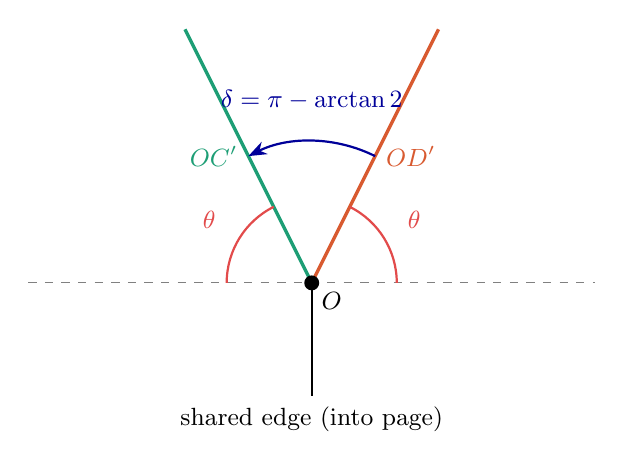
\begin{tikzpicture}[scale=1.8]
  % Side view of the fold
  \coordinate (O) at (0,0);
  \coordinate (flat1) at (-2, 0);
  \coordinate (flat2) at (2, 0);

  % Folded edges
  \pgfmathsetmacro{\foldang}{63.4349}
  \coordinate (up1) at ({-2*cos(\foldang)}, {2*sin(\foldang)});
  \coordinate (up2) at ({2*cos(\foldang)}, {2*sin(\foldang)});

  % Flat (original) edges
  \draw[gray, dashed, thin] (flat1) -- (O) -- (flat2);

  % Folded edges
  \draw[pent2, very thick] (O) -- (up1) node[midway, left, font=\small] {$OC'$};
  \draw[pent3, very thick] (O) -- (up2) node[midway, right, font=\small] {$OD'$};

  % Shared edge into page
  \draw[black, thick] (O) -- ++(0, -0.8) node[below, font=\small] {shared edge (into page)};

  % Dihedral angle arc
  \draw[blue!60!black, thick, -{Stealth}] ({1.0*cos(\foldang)}, {1.0*sin(\foldang)})
    arc ({\foldang}:{180-\foldang}:1.0);
  \node[blue!60!black, above, font=\small] at (0, 1.15) {$\delta = \pi - \arctan 2$};

  % Theta arcs
  \draw[vecred, thick] (0.6, 0) arc (0:{\foldang}:0.6);
  \node[vecred, font=\small] at ({0.85*cos(\foldang/2)}, {0.85*sin(\foldang/2)}) {$\theta$};

  \draw[vecred, thick] (-0.6, 0) arc (180:{180-\foldang}:0.6);
  \node[vecred, font=\small] at ({-0.85*cos(\foldang/2)}, {0.85*sin(\foldang/2)}) {$\theta$};

  % Vertex O
  \fill (O) circle (1.5pt);
  \node[below right, font=\bfseries\small] at (O) {$O$};
\end{tikzpicture}
\caption{Side view (looking along the shared edge). The folding angle $\theta =
\arctan 2$ and the dihedral angle $\delta = \pi - \arctan 2$ are supplementary.}
\label{fig:sideview}
\end{figure}

The folding angle $\theta = \arctan 2$ has an elegant interpretation in terms of the
golden ratio. Since
\[
  \cos\theta = \frac{1}{\sqrt{5}}, \qquad \sin\theta = \frac{2}{\sqrt{5}},
\]
we can also write $\tan\theta = 2$. The appearance of $\sqrt{5}$ is no coincidence:
it is intimately connected to the golden ratio $\varphi = (1+\sqrt{5})/2$, which
governs the geometry of the regular pentagon and, by extension, the dodecahedron.

The dihedral angle $\delta \approx 116.57^\circ$ is notably \emph{less} than
$120^\circ$, which is the angle at which three faces would meet to form a flat
surface. This small deficit of approximately $3.43^\circ$ per edge is what allows
the twelve pentagonal faces to close into a convex solid rather than tiling the plane.

%% ===================================================================
\section{Summary}
%% ===================================================================

We have derived the dihedral angle of the regular dodecahedron by:
\begin{enumerate}[nosep]
  \item Arranging three regular pentagons edge-to-edge in a plane, sharing a common
        vertex $O$.
  \item Rotating Pentagons~2 and~3 about their shared edges $OA$ and $OB$ by angle
        $\theta$, using Rodrigues' rotation formula.
  \item Exploiting the mirror symmetry of the configuration to reduce the vector
        equation $C'(\theta) = D'(\theta)$ to a single scalar equation.
  \item Solving analytically to obtain $\cos\theta = 1/\sqrt{5}$, i.e.,
        $\theta = \arctan 2$.
  \item Verifying numerically to machine precision.
\end{enumerate}

The dihedral angle is therefore:
\[
  \boxed{\delta = \pi - \arctan 2 \approx 116.565^\circ.}
\]

\end{document}
